\section*{Convolutional Neural Networks}

\textbf{CNNs} are a special kind of neural network designed to process data with a grid-like topology. Examples: time series data (1-D grid), images (2-D grid), etc. They employ a mathematical operation called \textbf{convolution} in \textit{at least one} of their layers.

\section*{Convolution}

\begin{figure}[H]
  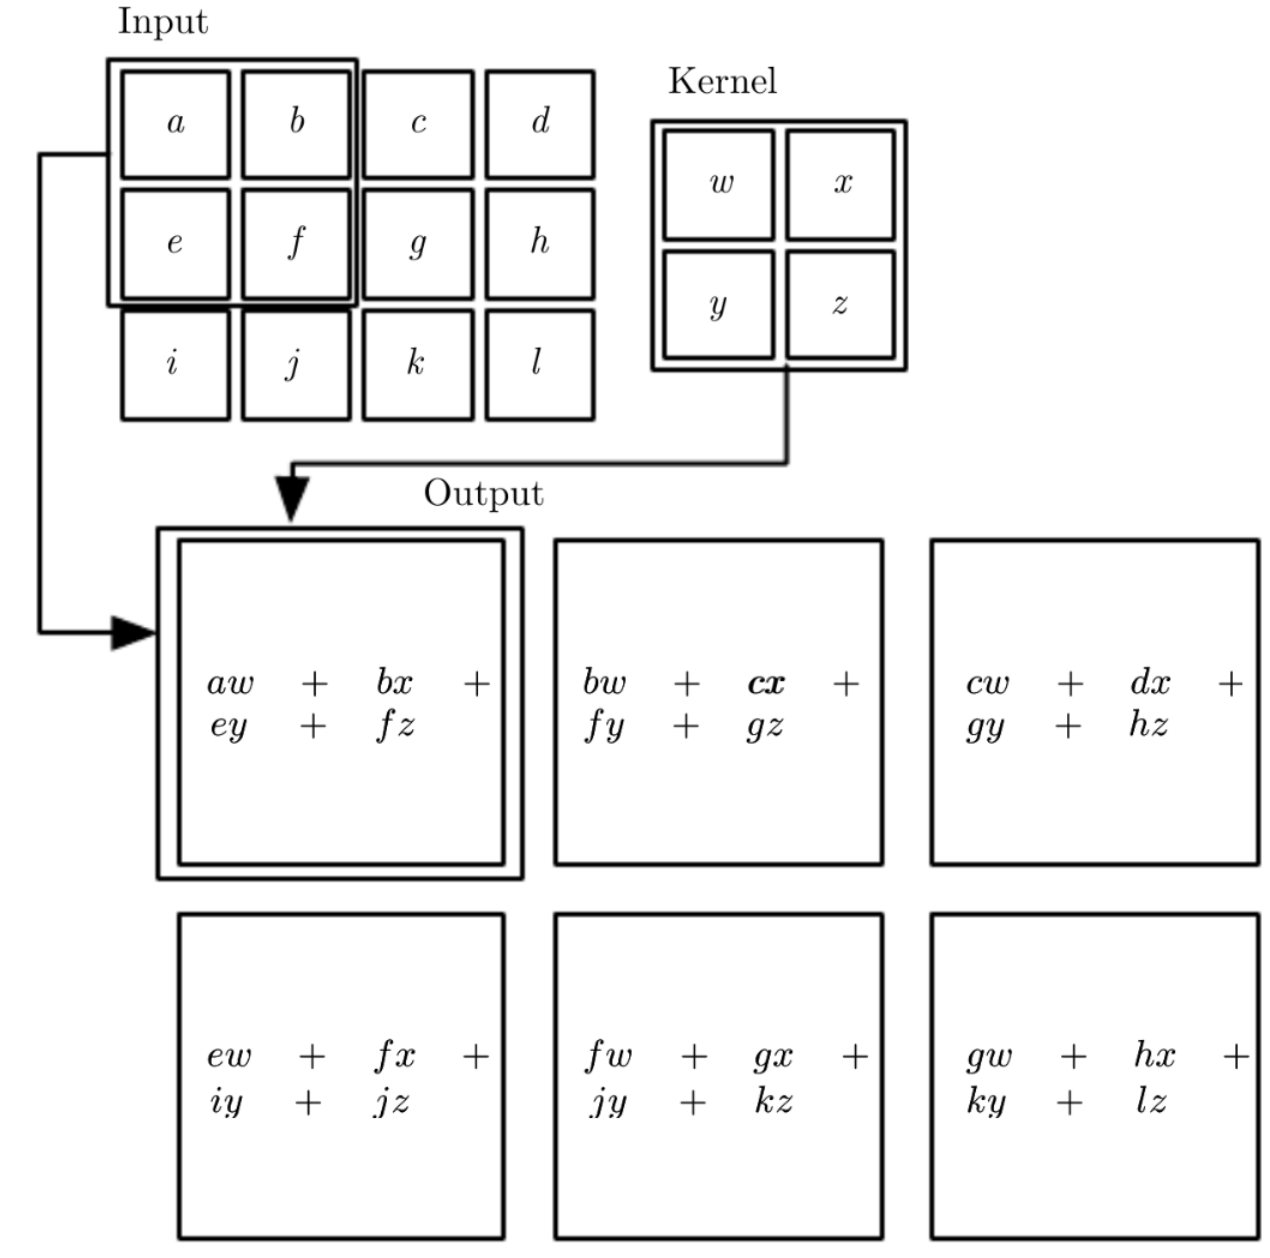
\includegraphics[width=\linewidth]{images/convolution.png}
\end{figure}

\textbf{Why convolution?} Convolution leverages three important ideas that improve a machine learning system:

\begin{itemize}
  \item \textbf{Sparse Interactions:} In traditional MLPs, every output neuron interacts with every input neuron. CNNs typically have sparse connectivity. This is accomplished by making the kernel smaller than the input.
  \item \textbf{Parameter Sharing:} Refers to using the same parameter for more than one function in a model. In an MLP, each weight is used only once. In CNNs, the same kernel is used across the entire input. 

  \item \textbf{Equivariant Representations:} Equivariance means that if the input changes, the output changes in the same way. Mathematically, a function $f$ is equivariant to a function $g$ if $f(g(x)) = g(f(x))$ $\forall$ inputs $x$.
    \begin{itemize}
      \item In image classification, if an image is shifted, the output of a convolutional layer shifts in the same way. \textbf{Convolution is not equivariant to rotation or scaling.}
      \item In time series analysis, if an event is shifted to later in time, the same features will be detected, just at a later time.
    \end{itemize}
\end{itemize}

The output of convolution is called a \textbf{feature map}.

\subsubsection*{Padding}

A common problem with convolution is that it reduces the size of the output. $I_{5 \times 5} * K_{3 \times 3} = O_{3 \times 3}$ ($I \rightarrow$ Input, $K \rightarrow$ Kernel, $O \rightarrow$ Output). This is resolved by \textbf{padding}, which adds extra pixels around the input image. The most common type is \textbf{zero padding}.

\begin{figure}[H]
  \centering
  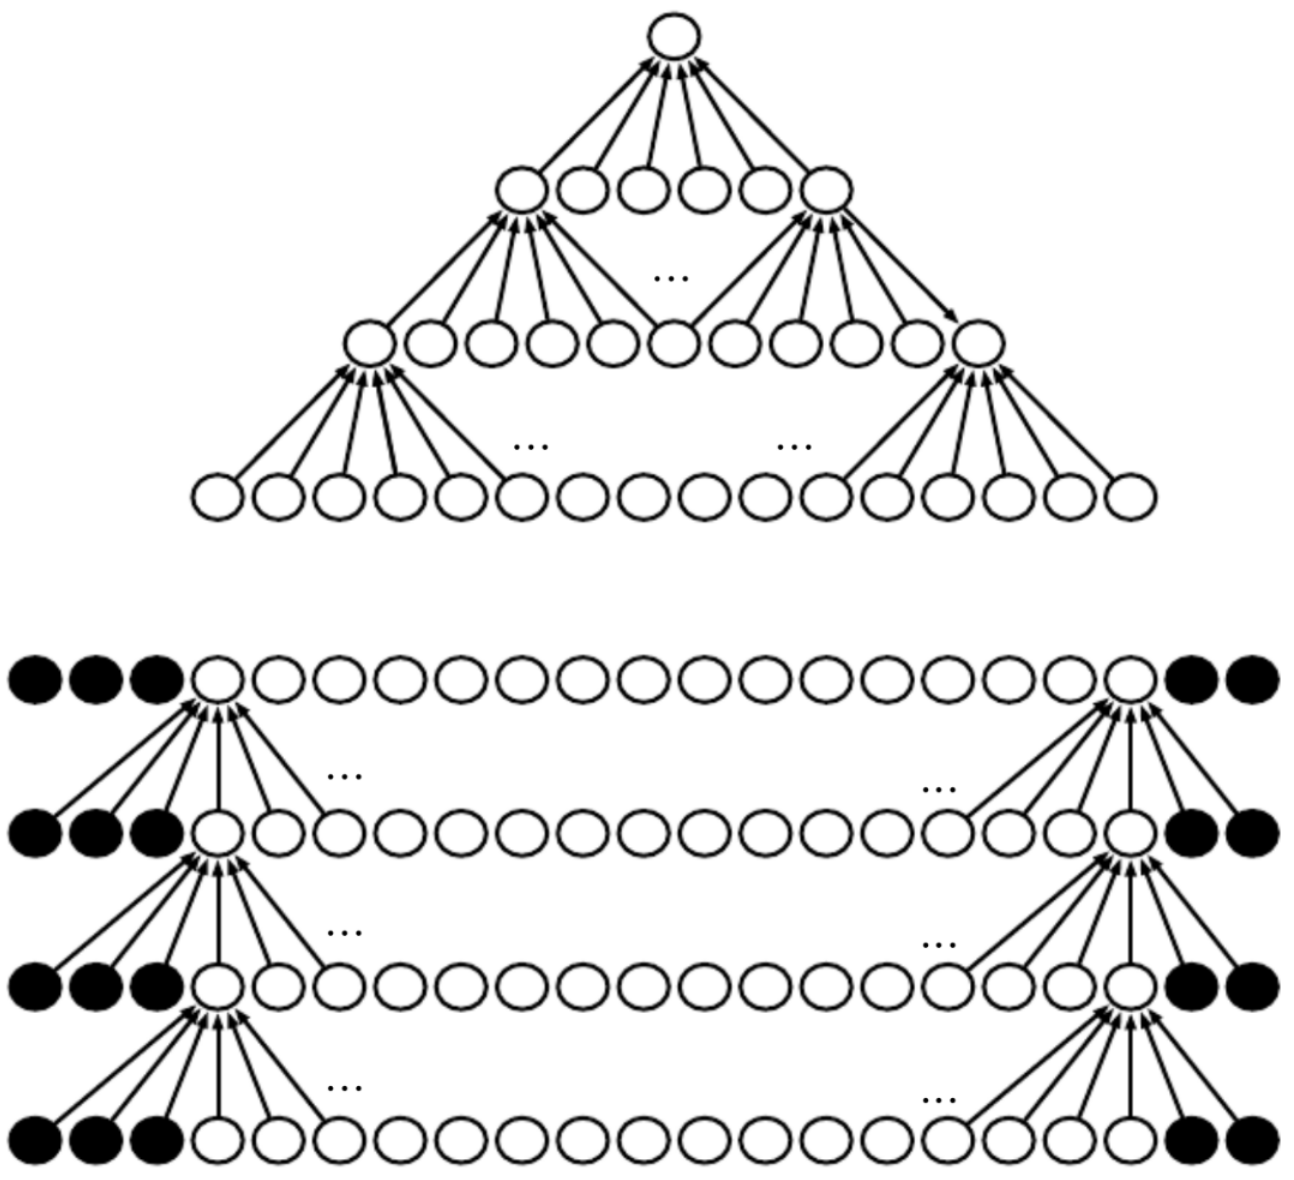
\includegraphics[width=\linewidth]{images/zero_padding.png}
  \caption{Effect of zero padding on the network size.\\ \textbf{Top:} no zero padding, representation shrinks by 5 pixels at each layer. \textbf{Bottom:} with zero padding, representation remains the same size.}
\end{figure}

\subsubsection*{RGB Convolution}

RGB images are composed of three channels: red, green, and blue. Each channel is a 2D grid of pixels. When we apply convolution to an RGB image $I$, we use a 3D kernel that has the same depth as the number of channels in $I$.

\begin{figure}[H]
  \centering
  \includegraphics[width=\linewidth]{images/rgb_convolution.png}
\end{figure}

\subsubsection*{Strided Convolution}

Sometimes we want to skip over some positions of the input data in order to reduce the computational cost, We can think of this as downsampling the output of the full convolution function. The number of positions to skip is called the \textbf{stride} of the convolution.

\begin{figure}[H]
  \centering
  \includegraphics[width=0.8\linewidth]{images/strided_convolution.png}
  \caption{Strided Convolution is equivalent to downsampling the output of a full convolution.}
\end{figure}

Size of the feature map ($W_\text{out}$) obtained after a convolution with stride $s$ is given by:

\begin{equation*}
  W_\text{out} = \bigg\lfloor \frac{W_\text{in} - F + 2P}{s} \bigg\rfloor + 1
\end{equation*}

where $W_\text{in} \rightarrow$ input image width, $F \rightarrow$ filter size, $P \rightarrow$ padding, and $s \rightarrow$ stride.
\subsection*{Pooling}

A pooling function replaces the output of the net at a certain location with a summary statistic of the nearby outputs. Most common: \textbf{max pooling}, which takes the maximum value in a region. Others: average, weighted average, L2 norm, etc.

\subsection*{Layers in CNNs}

\begin{itemize}
  \item \textbf{Convolutional Layer:} Applies a convolution operation to the input.
  \item \textbf{Activation Function:} Applies a non-linear activation function (e.g., ReLU) to the output of the convolutional layer.
  \item \textbf{Pooling Layer:} Reduces the spatial dimensions of the input (e.g., max pooling).
  \item \textbf{Fully Connected Layer:} Connects every neuron in one layer to every neuron in the next layer, typically used at the end of the network for classification tasks.

    The activation function used at the output layer depends on the task: (i) for binary classification, \textbf{sigmoid} activation; (ii) for multi-class classification, \textbf{softmax} activation, etc.
\end{itemize}

\subsection*{CNN Architecture}

\begin{figure}[H]
  \centering
  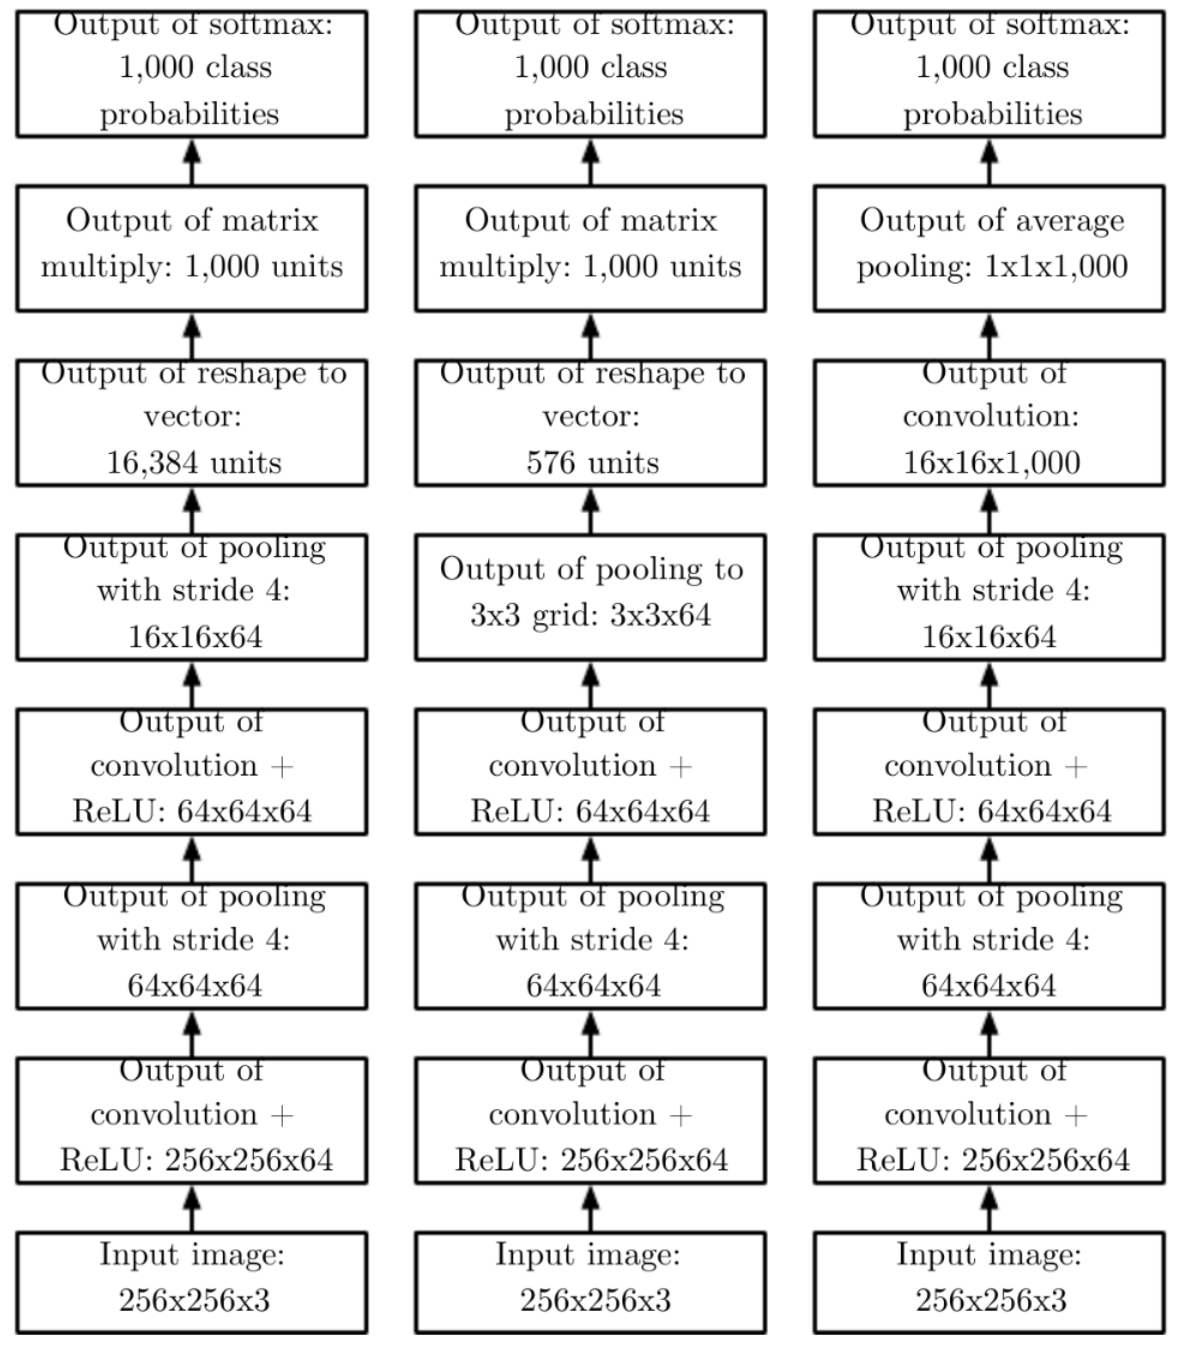
\includegraphics[width=\linewidth]{images/cnn_architecture.png}
  \caption{Typical architectures of CNNs}
\end{figure}

\subsection*{Common CNN-Based Architectures}

\subsubsection*{LeNet}

LeNet is one of the earliest CNN architectures, designed for handwritten digit recognition. It consists of 2 convolutional layers, 2 pooling layers, and 3 fully connected (FC) layers.

\begin{figure}[H]
  \centering
  \includegraphics[width=\linewidth]{images/lenet.png}
\end{figure}

\subsubsection*{AlexNet}

AlexNet is a relatively shallow architecture with 5 convolutional layers, 3 pooling layers, 2 FC layers and a softmax output layer.

\begin{figure}[H]
  \centering
  \includegraphics[width=\linewidth]{images/alexnet.png}
\end{figure}

\subsubsection*{VGGNet}

The VGGNet architecture is characterized by a building block of \textbf{two convolutional layers} (both ReLU) followed by a \textbf{max pooling layer}. At the end, there are several \textbf{fully connected layers} also using ReLU activation. The final layer uses softmax activation for classification.

\begin{itemize}

  \item The key architectural feature is the use of small $3 \times 3$ convolutional filters, which allows for deeper networks while maintaining a manageable number of parameters.

  \item Three VGG models, VGG-11, VGG-16, and VGG-19; were proposed the models had 11, 16, and 19 layers.

  \item All versions of the VGG models ended the same with three fully connected layers. However, the number of convolution layers varied VGG-11 contained 8 convolution layers, VGG-16 had 13 convolution layers, and VGG-19 had 16 convolution layers.

\end{itemize}

\begin{figure}[H]
  \centering
  \includegraphics[width=\linewidth]{images/vgg16.png}
\end{figure}

\subsubsection*{ResNet}

A common problem with deep CNNs is that as the depth is increased, the accuracy gets saturated and starts degrading rapidly. This is due to the \textbf{vanishing gradient problem}. ResNet solves this by introducing \textbf{skip connections}.

\begin{itemize}
  
  \item \textbf{Skip Connections:} Consider an input $x$ and a series of transformations to produce $f(x)$. Core idea: with skip connections, instead of mapping $x \rightarrow y$ with a function $f(x)$, we map $x \rightarrow y$ with a \enquote{residual function} $f(x) = H(x) - x$.

  \item One of the major benefits of ResNet is that it allows for training very deep networks (e.g., 100+ layers) without suffering from the vanishing gradient problem.

\end{itemize}

\begin{figure}[H]
  \centering
  \includegraphics[width=\linewidth]{images/resnet.png}
\end{figure}
